\documentclass{article}
\usepackage{xeCJK}
\setCJKmainfont{Hiragino Mincho Pro}  % macOSの日本語フォント
\usepackage{amsmath}
\usepackage{amssymb}
\usepackage{amsfonts}
\usepackage{graphicx}
\usepackage{color}
\usepackage{bm}

%%%%%%%%%%%%%%%%%%%%%%%%%%%%%%%%%%%%%%%%%%%%%%%%%%%%%%%%%%%%%%%%%%%%%%%%%%%
% format 
%%%%%%%%%%%%%%%%%%%%%%%%%%%%%%%%%%%%%%%%%%%%%%%%%%%%%%%%%%%%%%%%%%%%%%%%%%%
\setlength{\oddsidemargin}{0.455cm} 
\setlength{\evensidemargin}{0.455cm} 
\setlength{\textwidth}{15.5cm} 
\setlength{\textheight}{22.54cm}
\setlength{\headheight}{0mm}
\setlength{\headsep}{0mm}
\setlength{\topskip}{0mm}
\setcounter{topnumber}{100}
\setcounter{bottomnumber}{100}
\setcounter{totalnumber}{100}
\renewcommand{\topfraction}{1.0}
\renewcommand{\bottomfraction}{1.0}
\renewcommand{\textfraction}{0.0}
\renewcommand{\floatpagefraction}{0.0}
\renewcommand{\baselinestretch}{1.0}
\pagestyle{empty}

%%%%%%%%%%%%%%%%%%%%%%%%%%%%%%%%%%%%%%%%%%%%%%%%%%%%%%%%%%%%%%%%%%%%%%%%%%%
% math symbols and commands
%%%%%%%%%%%%%%%%%%%%%%%%%%%%%%%%%%%%%%%%%%%%%%%%%%%%%%%%%%%%%%%%%%%%%%%%%%%
\newcommand{\eq}[1]{(\ref{#1})}
\newcommand{\mtx}[2]{\left[\begin{array}{#1} #2 \end{array}\right]}
\newcommand{\mycase}[1]{\left\{\begin{array}{ll} #1 \end{array} \right.}
\newcommand{\mb}[1]{\mbox{\boldmath$#1$}}
\newcommand{\lw}[1]{\smash{\lower2.ex\hbox{#1}}}
\newcommand{\zero}{\mathbf{0}}
\newcommand{\one}{\mathbf{1}}
\newcommand{\eps}{\varepsilon}

%%%%%%%%%%%%%%%%%%%%%%%%%%%%%%%%%%%%%%%%%%%%%%%%%%%%%%%%%%%%%%%%%%%%%%%%%%%
% colors
%%%%%%%%%%%%%%%%%%%%%%%%%%%%%%%%%%%%%%%%%%%%%%%%%%%%%%%%%%%%%%%%%%%%%%%%%%%
\newcommand{\myred}[1]{\textcolor{red}{#1}}
\newcommand{\myredbf}[1]{\textcolor{red}{\bf #1}}
\newcommand{\myblue}[1]{\textcolor{blue}{#1}}
\newcommand{\mybluebf}[1]{\textcolor{blue}{\bf #1}}
\newcommand{\mydarkblue}[1]{\textcolor[rgb]{0.0,0.0,0.5}{#1}}
\newcommand{\mygreen}[1]{\textcolor[rgb]{0.0,0.5,0.0}{#1}}
\newcommand{\mygreenbf}[1]{\textcolor[rgb]{0.0,0.5,0.0}{\bf #1}}
\newcommand{\mypurple}[1]{\textcolor[rgb]{0.5,0.0,0.5}{#1}}
\newcommand{\mypurplebf}[1]{\textcolor[rgb]{0.5,0.0,0.5}{\bf #1}}

\begin{document}
%%%%%%%%%%%%%%%%%%%%%%%%%%%%%%%%%%%%%%%%%%%%%%%%%%%%%%%%%%%%%%%%%%%%%%%%%%%
% ここからがレポートの記述
%%%%%%%%%%%%%%%%%%%%%%%%%%%%%%%%%%%%%%%%%%%%%%%%%%%%%%%%%%%%%%%%%%%%%%%%%%%

\begin{center} 
{\large \bf 知能プログラミング演習I 第2回レポート}
\end{center} %

\begin{flushright} 
\today % Date
\hskip 1mm
学籍番号 35714121 % 学籍番号
\hskip 1mm
氏名 福富隆大% 氏名
\end{flushright} % Name

%%%%%%%%%%%%%%%%%%%%%%%%%%%%%%%%%%%%%%%%%%%%%%%%%%%%%%%%%%%%%%%%%%%%%%%%%%%
\section{実験設定}
本実験では、MNISTデータセットの手書き数字(0〜2)を分類する深層ニューラルネットワークを実装した。
ネットワークの基本構成は以下の通りである:

\begin{itemize}
  \item 入力層:784ユニット(28×28ピクセルの画像)
  \item 第1中間層:100ユニット、活性化関数はReLU
  \item 第2中間層:50ユニット、活性化関数はReLU
  \item 第3中間層:10ユニット、活性化関数はReLU
  \item 出力層:3ユニット(クラス数)、活性化関数はソフトマックス
\end{itemize}

学習率は$\eta = 10^{-2}/\text{epoch}$とし、エポック数は50とした。
訓練データとテストデータはMNISTデータセットから、クラス0, 1, 2のみを抽出して使用した。

また、以下の実験を行った:
\begin{enumerate}
  \item 基本設定での学習と評価
  \item 活性化関数の比較実験:ReLU、シグモイド関数、ハイパボリックタンジェントを使用した場合の比較
  \item 中間層のユニット数を変更した実験:(50-25-5)と(200-100-20)の2種類の構成で比較
\end{enumerate}
%%%%%%%%%%%%%%%%%%%%%%%%%%%%%%%%%%%%%%%%%%%%%%%%%%%%%%%%%%%%%%%%%%%%%%%%%%%


%%%%%%%%%%%%%%%%%%%%%%%%%%%%%%%%%%%%%%%%%%%%%%%%%%%%%%%%%%%%%%%%%%%%%%%%%%%
\section{結果}
\subsection{基本設定での学習結果}
図\ref{fig:error}に訓練誤差とテスト誤差の推移を示す。エポックが進むにつれて誤差が減少し、約20エポック後に収束している。最終的なテスト誤差は約0.1であった。

\begin{figure}[htbp]
  \centering
  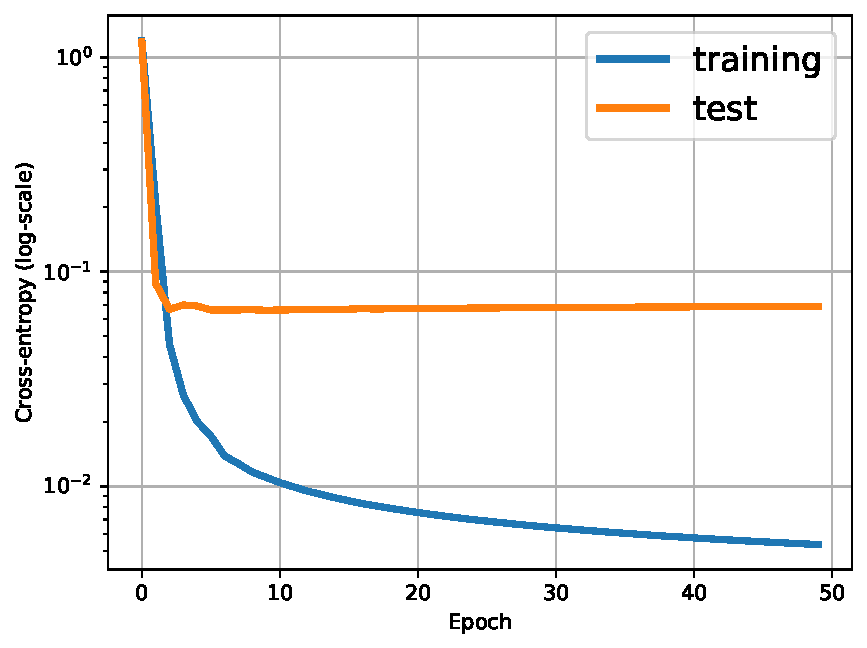
\includegraphics[width=0.8\textwidth]{error.pdf}
  \caption{訓練誤差とテスト誤差の推移}
  \label{fig:error}
\end{figure}

図\ref{fig:confusion}に混同行列を示す。対角成分が大きく、非対角成分が小さいことから、高い分類精度が得られていることがわかる。特に、クラス0とクラス1の分類精度が高く、クラス2の分類精度がやや低い傾向が見られた。

\begin{figure}[htbp]
  \centering
  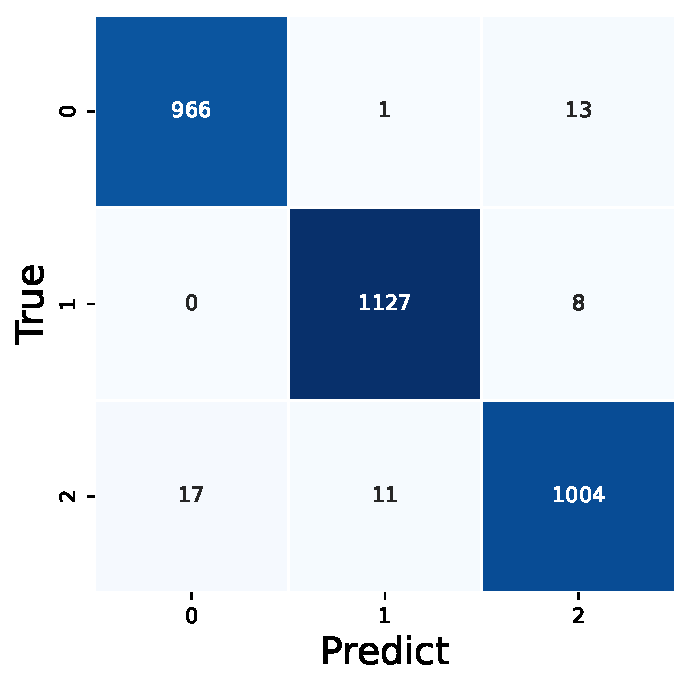
\includegraphics[width=0.5\textwidth]{confusion.pdf}
  \caption{混同行列}
  \label{fig:confusion}
\end{figure}

\subsection{活性化関数の比較}
図\ref{fig:activation_comparison}に、ReLU、シグモイド関数、ハイパボリックタンジェントを用いた場合の誤差推移を比較した結果を示す。ReLUが最も速く収束し、最終的な誤差も小さかった。シグモイド関数は学習の初期段階では誤差の減少が遅いが、最終的にはReLUに近い性能を示した。ハイパボリックタンジェントはReLUとシグモイド関数の中間的な挙動を示した。

\begin{figure}[htbp]
  \centering
  \includegraphics[width=0.8\textwidth]{activation_comparison.pdf}
  \caption{活性化関数による誤差推移の比較}
  \label{fig:activation_comparison}
\end{figure}

\subsection{中間層のユニット数の比較}
図\ref{fig:units_comparison}に、中間層のユニット数を変更した場合の誤差推移を比較した結果を示す。基本設定(100-50-10)と比較して、ユニット数を減らした場合(50-25-5)は学習が速く収束するが、最終的な誤差はやや大きくなった。一方、ユニット数を増やした場合(200-100-20)は学習が遅いが、最終的な誤差は小さくなった。

\begin{figure}[htbp]
  \centering
  \includegraphics[width=0.8\textwidth]{units_comparison.pdf}
  \caption{中間層のユニット数による誤差推移の比較}
  \label{fig:units_comparison}
\end{figure}
%%%%%%%%%%%%%%%%%%%%%%%%%%%%%%%%%%%%%%%%%%%%%%%%%%%%%%%%%%%%%%%%%%%%%%%%%%%


%%%%%%%%%%%%%%%%%%%%%%%%%%%%%%%%%%%%%%%%%%%%%%%%%%%%%%%%%%%%%%%%%%%%%%%%%%%
\section{考察}
\subsection{活性化関数の影響}
ReLUは勾配消失問題が起きにくく、計算も単純なため、学習が効率的に進んだと考えられる。一方、シグモイド関数は出力が0から1の間に制限されるため、深い層では勾配消失問題が発生しやすく、学習が遅くなったと考えられる。ハイパボリックタンジェントは出力が-1から1の間に制限されるため、シグモイド関数よりも勾配消失問題が緩和され、中間的な性能を示したと考えられる。

\subsection{ネットワーク構造の影響}
中間層のユニット数を増やすと表現力が向上するが、過学習のリスクも高まる。本実験では、基本設定(100-50-10)が最もバランスが良く、高い分類精度を示した。ユニット数を減らした場合(50-25-5)は、モデルの表現力が不足し、複雑なパターンを学習できなかった可能性がある。一方、ユニット数を増やした場合(200-100-20)は、表現力は向上するが、学習に時間がかかり、過学習のリスクも高まる。

\subsection{誤分類の分析}
混同行列から、クラス2(数字の「2」)の分類精度がやや低いことがわかる。これは、「2」の形状が複雑で、書き方のバリエーションが多いためと考えられる。特に、「2」と「1」の混同が見られたが、これは「2」の上部が「1」に似ている場合があるためと推測される。

\subsection{総括}
深層ニューラルネットワークはMNISTデータセットの分類に高い精度を示した。特にReLUを活性化関数として用いた場合に良好な結果が得られた。また、ネットワークの構造(層の数やユニット数)も性能に大きく影響することがわかった。今後の課題としては、より複雑なデータセットでの評価や、正則化手法の導入による過学習の抑制などが考えられる。
%%%%%%%%%%%%%%%%%%%%%%%%%%%%%%%%%%%%%%%%%%%%%%%%%%%%%%%%%%%%%%%%%%%%%%%%%%%
% ここまでがレポートの記述
%%%%%%%%%%%%%%%%%%%%%%%%%%%%%%%%%%%%%%%%%%%%%%%%%%%%%%%%%%%%%%%%%%%%%%%%%%%
\end{document}
